\section{Durchführung der Anforderungsanalyse}
\subsection{Stakeholderanalyse}
Nachdem bereits geklärt wurde, wie eine Stakeholderanalyse durchgeführt werden kann, soll diese nun auch für das Projekt beschrieben werden.
Das Brainstorming hat ergeben, dass in erster Linie die \textbf{Benutzer} des Produkts sowie die \textbf{Erwerber} als Stakeholder in Betracht gezogen werden müssen.
Die Benutzer sind dabei vornehmlich männlich\autocite[vgl.]{Ailon.a} und in der Altersgruppe von 18 bis 40 Jahren anzusiedeln\autocite[vgl.]{Ailon.b}.
Zudem ist die \textbf{Organisation}, welche das Produkt entwickelt, sowie regulatorische Behörden ebenfalls als Stakeholder zu betrachten.

Darüber hinausgehende Stakeholder sind die \textbf{Rechteinhaber} der Filme, welche auf der Seite präsentiert werden sollen.
Da diese die Vorgaben machen, welche Sicherheitskriterien gegen Piraterie erfüllt werden müssen, sind diese ebenfalls als Stakeholder zu betrachten.

Die weiterführende Analyse der Dokumente hat ergeben, dass zusätzlich auch die \textbf{Investoren} in die Firma des Kunden Stakeholder sind.
Diese Geldgeber sind für die Finanzierung des Projekts verantwortlich und können dementsprechend Einfluss auf die Anforderungen nehmen.
Ebenso sind \textbf{regulatorische Behörden} zu berücksichtigen, da diese die Einhaltung der gesetzlichen Vorgaben überprüfen.

Die Analyse der Produktentwicklung hat zuletzt noch ergeben, dass auch die \textbf{Entwickler} des Produkts als Stakeholder betrachtet werden müssen.
So sind diese dafür verantwortlich, dass das Produkt den Anforderungen entspricht und die Anforderungen in der Dokumentation korrekt beschrieben sind.

Somit ergeben sich folgende Stakeholder:
\begin{itemize}
    \item Benutzer
    \item Kunde/Erwerber
    \item entwickelnde Organisation
    \item Regulatorische Behörden
    \item Rechteinhaber
    \item Investoren
    \item Entwickler
\end{itemize}

Diese Personengruppen sollen nun anschließend in einer Stakeholderanalyse betrachtet werden.
Zuerst ist die Einordnung in die Power-Interest Matrix vorzunehmen.
\begin{figure}[ht]
    \centering
    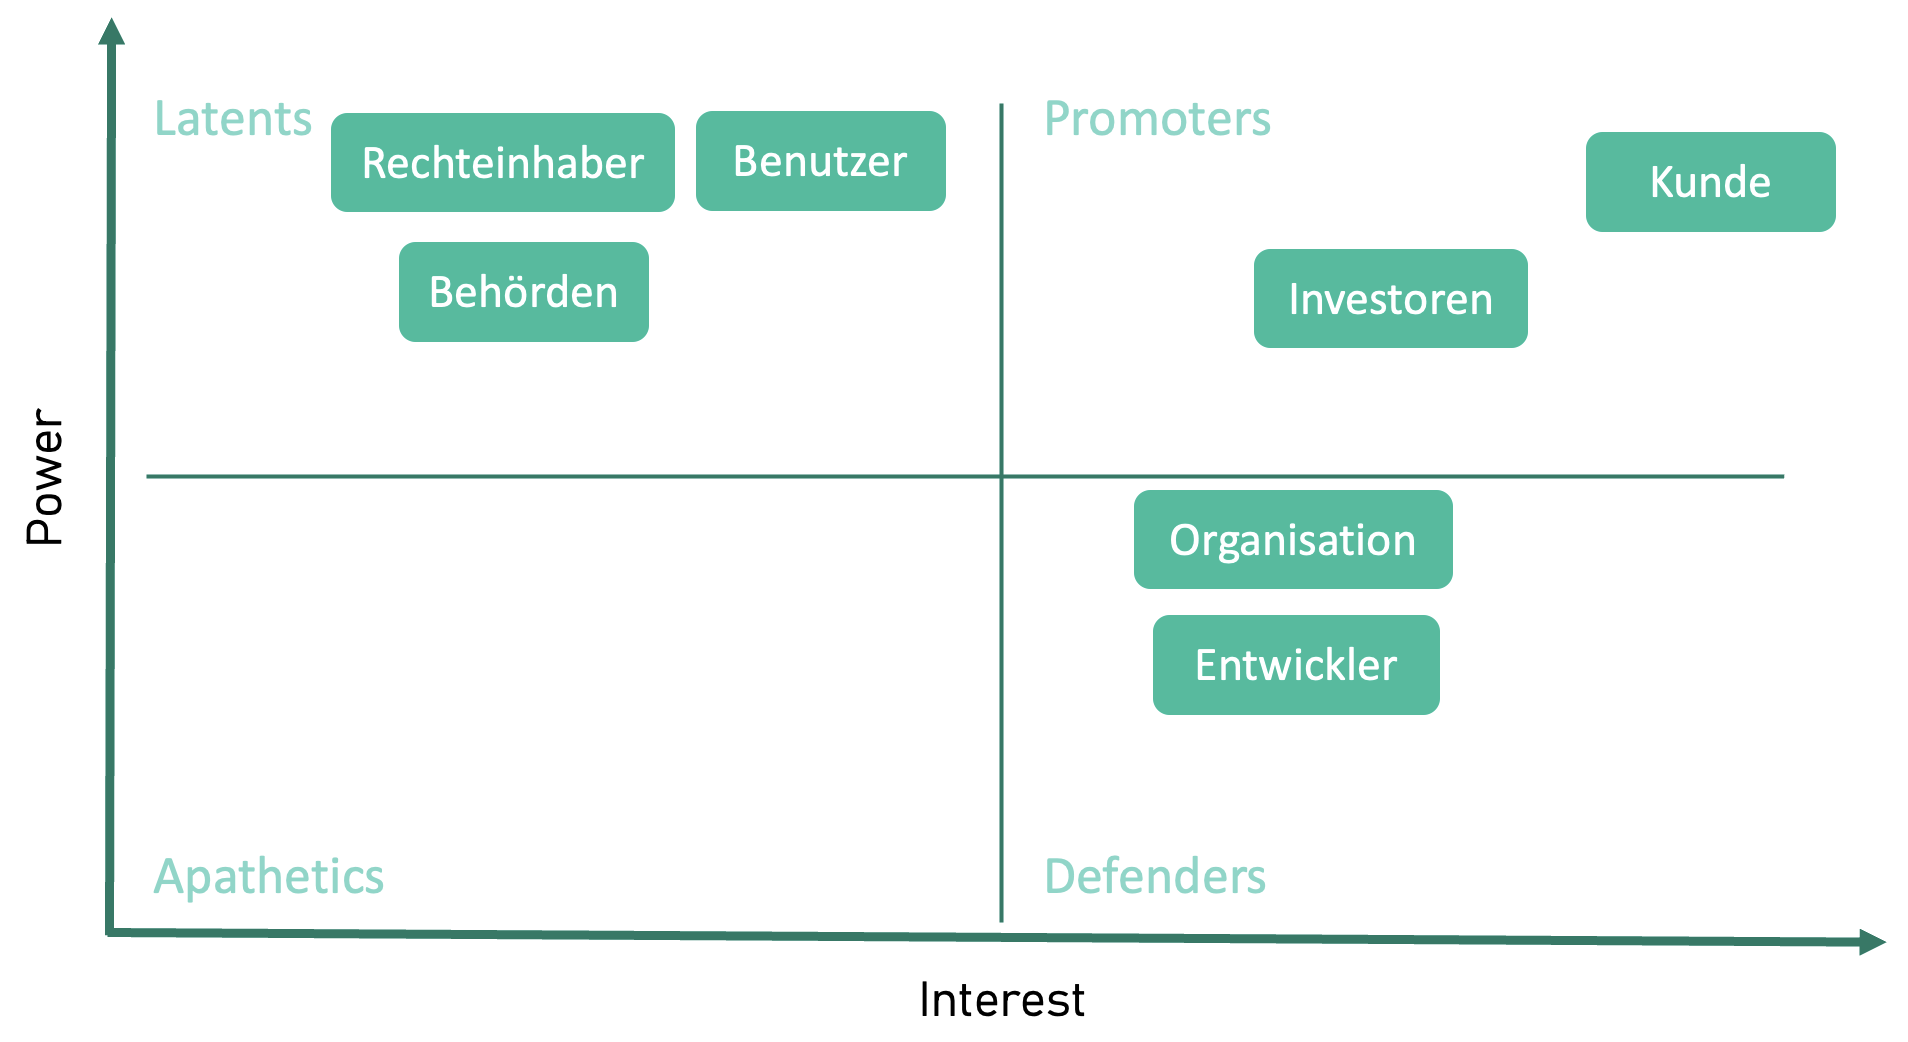
\includegraphics[width=0.7\textwidth]{Power-Interst-Matrix-Teil2}
    \caption{Power-Interest Matrix für die Stakeholderanalyse}
    \label{fig:power-interest-matrix2}
\end{figure}

Aus dieser geht hervor, dass die Kunden und die Investoren am meisten Macht sowie Interesse an dem Projekt haben.
Somit sollten diese sehr eng in das Projekt eingebunden werden und die Einwicklung des Produkts mitbestimmen.
Eine hohe Macht, ohne dabei ein besonders hohes Interesse zu haben, haben die regulatorischen Behörden, die Nutzer sowie die Rechteinhaber der Filme.
Alle drei Gruppen sind nicht direkt vom Ausgang der Entwicklung abhängig.
Die Benutzer beispielsweise haben auch Alternativen zum angebotenen Produkt, auch wenn dieses im optimalen Fall einen gewissen Mehrwert bieten soll.
Zuletzt sind die Entwickler sowie die Organisation, welche das Produkt entwickelt, in die Gruppe der Verteidiger einzuordnen.
Diese haben zwar ein hohes Interesse an dem Projekt, da Sie finanziell davon abhängig sind, jedoch bestimmt der Kunde über die Anforderungen an das Projekt.

%TODO: Hervorhebungsmodell?

Nun müssen die Stakeholder nach Ihren Anforderungen an das Produkt eingeteilt werden.
So ist für die Benutzer ein einfaches und intuitives Interface wichtig, sodass diese die Filme möglichst einfach finden und wiedergeben können.
Die Kunden sowie die Investoren hingegen sind an einem möglichst hohen Umsatz interessiert.
Deswegen ist es ihnen wichtig, dass zum einen die Kunden möglichst zufrieden sind, allerdings auch, dass die Entwicklungskosten möglichst gering sind.
Dies widerspricht sich allerdings mit dem Verständnis der entwickelnden Organisation und den Entwicklern, die eine hohe Qualität des Produkts anstreben.
Die regulatorischen Behörden sind an der Einhaltung der gesetzlichen Vorgaben interessiert, weshalb diese die Einhaltung der Sicherheitskriterien überprüfen wollen.
Zuletzt sind die Rechteinhaber an der Einhaltung der Sicherheitskriterien interessiert, da diese verhindern wollen, dass Kopien der Filme im Internet verbreitet werden.
